\documentclass{article}
\setlength{\headheight}{13.59999pt}
\usepackage[utf8]{inputenc}

\title{Luminosity function}
\author{Henrik Andrews}

\usepackage{natbib}


\usepackage[ portrait, margin=2cm]{geometry}
\usepackage{graphicx}
\usepackage{amsmath}
\usepackage{upgreek}
\usepackage{bbold}
\usepackage{fancyhdr}
\usepackage{mathtools}
\usepackage{tabularx}
\usepackage{lipsum}
\usepackage{pdfpages}
\setlength{\parindent}{0em}
\setlength{\parskip}{1em}
\usepackage{caption}
\usepackage{multicol}

\usepackage{float}
\newcommand{\HRule}[1]{\rule{\linewidth}{#1}}
\usepackage{listings}
\usepackage{color} %red, green, blue, yellow, cyan, magenta, black, white
\definecolor{mygreen}{RGB}{28,172,0} % color values Red, Green, Blue
\definecolor{mylilas}{RGB}{170,55,241}
\definecolor{backcolour}{rgb}{0.95,0.95,0.92}
\begin{document}

% title source: https://www.overleaf.com/project/6021d9e4632b9ef90aa8d238
\title{ \normalsize \textsc{AREA}
	\\ [2.0cm]
	\HRule{0.5pt} \\
	\LARGE \textbf{\uppercase{Theme}}		
	\\ Title\\
	\HRule{2pt} \\ [0.5cm]		
%fix the university logo !!!!!!!!!!!!!!!!!!!!!!!!
	\vspace{6cm}
	\begin{figure}[htp]
    \centering
    
\includegraphics[width=.2\textwidth]{Logo-Ntnu.svg.png}
    \end{figure}
	}

\author{
    \normalsize 
	\textbf{Henrik Døvle Andrews } \\
	Norwegian university of Science and Technology \\ 
}

\maketitle
\setcounter{page}{ 0 }

\newpage

\pagestyle{fancy}
\fancyhf{}
\setlength\headheight{12pt}
\fancyhead[L]{Henrik Døvle Andrews}
\fancyhead[R]{Luminosity functions}
\fancyfoot[R]{Page \thepage \:}
\setcounter{page}{1}
\bibliography{bib}
\bibliographystyle{apalike}

\maketitle

% Abstract
\begin{abstract}
\lipsum[1] % Replace with your abstract text
\end{abstract}

\newpage 
% Summary (you might use a simple section for this)
\section*{Summary}
\lipsum[2] % Replace with your summary text

\newpage
% Acknowledgments
\section*{Acknowledgments}
\lipsum[3] % Replace with your acknowledgment text

\newpage
% Table of Contents (optional)
\tableofcontents

\newpage
% List of Figures
\listoffigures

% List of Tables
\listoftables

-abstract 
-sammendrag
-acknowledgments
-list of figure
-list of tables


\section{Introduction}

\section{The ever expanding universe}
In order to investigate sources very far away from an observer it is important to understand the influence this distance has on your desired observable. Therefore in astrophysics and astronomy in general there are distances created to take into account the effects of an expanding universe. 


\subsection{comsographic parameters}

The most notorious parameter is the Hubble constant $H_0$. This parameter sets the recession speed of a point at proper distance d and our current position via this equation.
\begin{equation}
    v = H_0 d 
\end{equation}
The subscript $0$ refers to the present epoch since in general $H_0$ changes with time. The value of $H_0$ is quite debated so I will  follow the nomenclature of D. Hogg and write it as a parameterized equation. 
$$
H_0= 100\frac{km}{s}\frac{1}{Mpc} h 
$$
where $h$ is a dimensionless number that according to current knowledge  can take the value between $0.5$ to $0.8$  

The Hubble constant has units of inverse time and therefore one can define the Hubble time as 
$$
t_H = \frac{1}{H_0}
$$


The constant also has units of speed, and therefore we can define the Hubble distance. 

$$
D_H = \frac{c}{H_0}
$$

\subsection{Components of the universe}
In this paper and in most articles one refers to the flat lambda CDM model to parameterize the contents of the universe and by extension the properties of its expansion. Here two important parameters to define are the mass density of the universe $\rho_0$ and the cosmological constant $\Lambda$. These variables which change with time also define the metric tensor in general relativity and allow us to model the curvature of the universe given an initial configuration.  njaaa, skriv på nytt. 

One can write these into dimensionless variables as such

$$
\Omega_m = \frac{8\pi G\rho_0}{3H_0^2}
$$

$$
\Omega_\Lambda = \frac{\Lambda c^2}{3H_0^2}
$$



In general one has a third density parameter $\Omega_k$ which defines the curvature of spacetime and is defined from 

$$
\Omega_m + \Omega_\Lambda + \Omega_k = 1
$$



The flat lambda CDM has three components, the dark energy density, the dark matter density, and the ordinary matter parameter. In the rest of this paper and other articles used by this dissertation the values of these components are represented by their $\Omega$ parameter and one has a universe with $\Omega_\Lambda = 0.7$, and $\Omega_m = 0.3$ also known as the flat lambda since the curvature parameter is $0$


\subsection{Redshift}
Redshift is defined as the fractional Doppler shift of emitting light. The Doppler effect is a known effect on different observables in our universe where the relative motion of sources to observers will impact the observable. The redshift is quantified for a light source as 

\begin{equation}
    z = \frac{\nu_e}{\nu_o}-1 = \frac{\lambda_o}{\lambda_e}-1
\end{equation}

Here $o$ refers to the observed quantity and $e$ the emmited. 
If one want to connect this redshift to the velocity of the observed object one needs to go to general relativity. 
There is an analog in special but one omits it here since one does not use it.
The important factor is that redshift is an observable and can help us determine distances of objects. 
especially if they are far away the relative velocity becomes negligible and 
only the effect of the expansion of the universe become important. 


\subsection{Comoving distance}
The comoving distance or more clearly the line of sight distance for an observer locted here
 at earth is a foundational distance measure in cosmography. All other distance measures can be 
 derived from it. One derives it by defining the small co-moving distance $\delta D_c$. 
 This quantity defines the distance between two objects that remains constant when both objects expand with the Hubble flow.
  One can think of it as a proper distance from relativity since it is constant in all "time-frames". 
  If one wants the total comoving distance one integrates all $\delta D_c$ in the line of sight from $z= 0$ to the object. 
In order to do this one need to take into account the different densities in the universe, from  \cite{hogg2000distance} one defines the function 

\begin{equation}
    E(z)  = \sqrt{\Omega_m(z+1)^3 +\Omega_k (1+z)^2 + \Omega_\Lambda  }
\end{equation}


This function is defined by the density parameters defined above and also the redshift $z$. 
One can also relate this to the measured Hubble constant as measured by an hypothetical observer at 
redshift $z$ via $ H(z) = H_0 E(z)$. 


One then recives the comoving distance $D_c$ from 
\begin{equation}
    D_c =D_H \int_0^z\frac{dz}{E(z)}
\end{equation}
\subsection{Comoving distance part 2}
$D_c$ is the line of sight of an object and its observer but given different space-time geometry that line 
is distorted. If one looks a two objects, both at redshift z the distance between them will be given as as a 
function of the angle between them. If they are sperated by an angle $d\theta$ then the distance between them will be $d\theta D_m$ where $D_m$ is the comoving distance

%Therefore for different curvature, one need to map the geodesic onto our simplistic view. Therefore one gets the three different space geometry cases

$$
D_m =
\begin{cases}
  D_h\frac{1}{\sqrt{\Omega_k}}sinh(\frac{\sqrt{\Omega_k}D_c}{D_H}) & \text{if } \Omega_k > 0 \\
  D_c& \text{if } \Omega_k = 0 \\
  D_h\frac{1}{\sqrt{|\Omega_k|}}sin(\frac{\sqrt{|\Omega_k|}D_c}{D_H}) & \text{if } \Omega_k < 0
\end{cases}
$$

The different cases are dependent on the curvature of the universe, and one can see that one enters hyperbolic geometry or spherical geometry based on the different curvatures. The true curvature of the universe is still a mystery but recent studies suggest that it is flat, as expected. 


\subsection{Angular distance}


THe angul


\subsection{Luminosity distance}
The luminosity distance $D_l$ is defined through the relation between 
the bolometrix flux $F$ of a source and its bolometric luminosity $L$. 
The flux is the amount of energy per unit time per unit area and the luminosity is the total amount of energy per unit time. 
The luminosity distance is defined as
\begin{equation}
    D_l = \sqrt{\frac{L}{4\pi F}}
\end{equation}

In more clearer words it describes the total loss in energy due to lights travel across an expanding universe. 
The total observed flux an observer will see will be different from different distances.  the intrisic luminosity emmited at the source




It is related to the transverse comoving distance via 

\begin{equation}
    D_l = (1+z)D_m
\end{equation}

This of course is for bolometric quantities, but if one wants to calculate the spectral 
flux/ differential flux one need to take into account a correction. This correction comes 
from the fact that one is viewing a redshifted object. The object is emmiting in a different band than 
observed. The spectrum of the differnetial flux $F_\nu$ is related to the spectral luminosity via
\begin{equation}
    F_\nu = (1+z) \frac{L_{(1+z)\nu}}{L_\nu}\frac{L_\nu}{4\pi D_l^2}
\end{equation}

If one wishes to translate an observed spectral flux of particles to a density distriubtion one needs to take into account this redshift effect


\section{High energy particles}

\subsection{Cosmic rays and Neutrinios}

\subsection{Energy loss}

\subsection{Emissivity estimates}




\subsection{Emmision lines}
When a particle is photionized by the continuum radiation of a source it will emit a photon when it returns to its ground state. 
This photon will have a specific wavelength that is determined by the energy difference between the two states.
This wavelength is called the emmision line of the particle. When looking a dynamical systems with high velocities 
the doppler shift of these emmision lines becomes important since it will affect the observed spectra of the source.

https://lweb.cfa.harvard.edu/~pberlind/whipple/agn.html



\subsubsection{Broad emmision lines}
Broad emission lines in the case of AGN are formed from the high density gas clouds located close the the central black hole. The 
high density parameter is innferred from the fact that one only sees broad emission from permitted line transitions (f.ex hydrogen Lynman and Balmer,
iron II, and magnesium II).High densities allow for collisional de-exitation. And the boradaning is an indictation that these gas clouds are moving are moving 
at huge velocities around the massive objects. This implies that they are located close to the black hole
\subsubsection{Narrow emmision lines}
Narrow emission lines are on the other hand formed in low density gas clouds. The low densities are inferred from the fact that one sees
both permitted and forbbiden line transitions. They are narrow lines due to their velocities being substantially lower than the inner most gas clouds.


We will be discussing two types of neutrino generation. The pp chain and p$\gamma$ production
\section{Active galactic nuclei}




Active Galactic Nuclei (AGNs) is an interesting field in astrophysical studies. 
Since their discovery, there has been rapid advancement in understanding these phenomena.
Today, AGNs are known to be among the brightest entities in the night sky,
but they only gained significant attention in the 1950s. 
This shift occurred with the arrival of new radio observations, which revealed a new type of quasi stellar
object through the discovery of Quasars.

Initially, these luminous objects, characterized by broad, 
unidentifiable spectral lines, were enigmatic to scientists in the early 1960s. 
However, with the identification of more sources and their optical parts, 
it became clear that these were not stars but a distinct class of celestial objects. 
Research done by M. Schmidt on of the emission lines from 
the Quasar 3C 273 opened the interpretation of these celestial objects. 
He found that the emmision lines of quasars were similar to hydrogen, but were redshifted by a factor of 0.158,
an exceptionally high value at the time \cite{Shields_1999}. Observations at the same time also revealed significant 
variability in quasar luminosity, suggesting that these objects were no larger than one light year across. 

These observations lead to the speculation of super luminous objects located very far away from earth. The problem was that such objects
had no reasonable explaination at the time. It was not until the mid 1960 early 1970s when modern cosmology was 
afoot that more of these issues were resolved.

Observation of the surrounding galaxy of AGNs with matching redshift and observation of gravitational lensing cemented 
the distances of these objects. In addition the modern view of black holes which had only been a theory in the 1950s came to
furition and the modern model of a AGN was born. This modern perspective views AGNs as supermassive black holes that
accrete matter from surrounding accretion disks. This accretion releases large amounts of energy and has also according to 
processes such as  the Blandford-Znajek process (1977), been shown to produce relativistic jets, when the black hole is rotating.

In the most recent times a landmark achievement was achieved in March 2021, when scientists associated with the Event Horizon Telescope project 
presented the first image of the supermassive black hole at the center of the Messier 87 galaxy, located 55 million light-years away.
This image, showing a bright ring surrounding a dark central region, aligns with predictions for an accreting supermassive black hole, 
reinforcing our understanding of these powerful cosmic sources.



\subsection{AGN structure and classification}


The modern view of AGNs is  unified model that combined different categories of powerful luminous objects viisble in the night sky.
These distinctions that astronomers made still
have value, but to understand an AGN it is important to get a picture of the modern structure of an AGN

An active galatic nucleous i defined as a galaxy containing a massive accreting black hole. This mass acording to \cite{Netzer_2015} 
is defined as $M_{BH} > 10^5 M_\odot$. AGNs aslo containt an Eddington ratio exceeding
the limit of $\frac{L_{AGN}}{L_{Edd}} = 10^{-5}$, where $L_{AGN}$ is the bolometric luminosity, and $L_{Edd}$ is the Eddington luminosity for a solar 
composition gas. These definitions are help constrain what galaxies might contain an AGN, f.ex it exludes the milky way 
by these criteria, but it failes to capture the full structure definition of an AGN. 
Therefore the structure of most AGNs will include several of the following components. 

\begin{itemize}
    \item A close rotational dominated accretion disc around the SMBH. The thickness defining this accretion flow will distinguish different AGNs. 
    One examples is an optiacl thin accretion disks that sometimes become advenction dominated.
    These flows will be referred to as radiation inefficient accretion flows(RIAF) due to the special nature of the disk.
    \item high density gas clouds that are said to be dust free moving at high velocities close to the black hole, in the so called broad line region(BLR)
    \item Low density gas clouds that move at lower velocities further away from the black hole in the so called narrow line region(NLR)
    \item A axisymmetric structure of dust that is responsible for the obscuration of the central region of the AGN. This is called the torus.
     It lies at a luminosity depended distance from the SMBH, but according to \cite{Netzer_2015} this is around 0.1 - 10 pc depending on the luminosity.
    \item A relativisitc jet that is powered by the accretion disk. This is not always present but is a common feature of AGNs.


\end{itemize}
The reader is directed to image \ref{fig:my_label} for a visual representation of the different components.


\begin{figure}
    \centering
    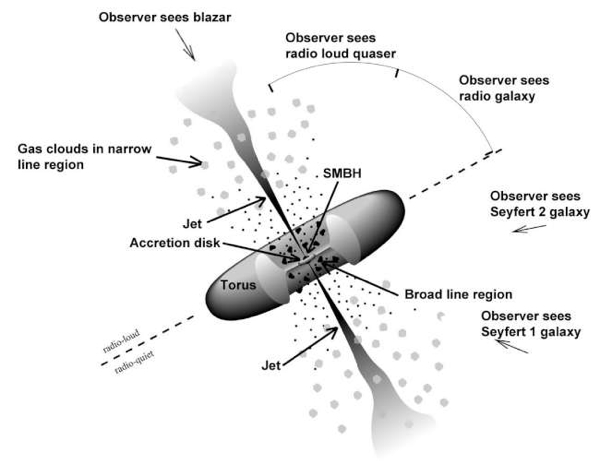
\includegraphics[width = 0.5\textwidth]{unified model agn.jpg}
    \caption{AGN unification}
    \label{fig:my_label}
\end{figure}

\subsubsection{Accretion disk}
An accretion disk is a natural consquence of the consveration of angular momentum. In the case for innfalling 
matter comming close to a super massiv black hole, the matter will have some angular momentum. This angular momentum would in a 
an ideal fluid orbit the black hole at some stable distance. Du to radative procesess and some fluid viscosity in this high density matter
the matter will lose angular momentum and spiral inwards. This inward spiral will eventually allow the matter to fall onto the black hole. 
This process of insprial is what is called accretion and the forces acting on the matter to cause the inspiral 
will also in the same process heat it up to high energies causing it to radiate. This radiation is closly linked to the 
infalling matter that is accreted onto the black hole and one can express the total luminosity of the accretion disk as 

\begin{equation}
    L_{acc} = \eta \dot{M}c^2
\end{equation}

Here $\eta$ is the efficiency of the accretion disk, $\dot{M}$ is the mass accretion rate and $c$ is the speed of light.

The efficiency of the accretion disk is a function of the spin of the black hole and the radius of the innermost stable circular orbit (ISCO).
The ISCO is a counter intruitve term in classical mechanics but in general relativity the maximum speed of a particle 
in addtion to a energy term in the calculationg of the orbit set bounds for how close a particle can be to 
a black hole without spiraling in. without going into to much detail the ISCO will be a solution of this equation based on the black holes mass and spin $a$

\begin{equation}
    6\frac{M}{r}-8\frac{aM^(\frac{1}{2})}{r^{3/2}}+3\frac{a^2}{r^2} = 1
\end{equation}

The accretion disk also has a bound for its maximum luminosity. As calculated for stars the Eddington
luminosity sets a maximum strength for the radiation pressure of the accretion disk. This is given as

Get sources!

\begin{equation}
    L_{Edd} = \frac{4\pi G M m_p c}{\sigma_T}
\end{equation}


write about BB radiation from accretion disk which give rise to x-rays. 

\subsubsection{Corona}

\subsubsection{dust torus}
mabye write about thermal radiation from dust torus

\subsubsection{Broad line region}
mabye write about BLR


\subsubsection{Jets}
Write about shock structure
write about non thermal radiation
Jet acceleration?, acceleration before jet, cooling effects



section radiation




\subsection{Types of AGNs}

https://astrobites.org/guides/galaxy-and-agn-types/

Before the unification of the AGNs astornomers named the pusseling objects based on their observational properties. These 
names are still used to this day and are somewhat usfull since their observational properties are important parameters for further study. 
The different classification are important in understanding which objects could have the potential to produce the different oberservables one 
looks for in the night sky. There is a lot of talk around AGNs being possible sources for ultra high energy comsic rays (UHECRs) and neutrinos.
This is yet to be comfirmed, but the theoretical framework for the neceassary particle acceleration is there. therefore is seems appropriate to
discuss the different types of AGNs and their observational properties.

\subsubsection{Type I and II AGNs}
One distinguishes type I and type II AGNs based on the presence of broad emission lines. In other words this distinction is
a matter of a visible nucleous or not. Type I refers to sources whose nucleus is exposed to the observer and whos spectrum is 
has both narrow and broad emmision lines. Type II refers to sources whose nucleus is obscured by a torus and therefore only has narrow emission lines.

\subsubsection{Blazars}
The most extreme class of AGN. These sources are distinuished by their relativistic jets that are pointed towards the observer. 
This jet produce both synchrotron and Inverse Compton gamma rays and are extremyl varaible over short timescales. The
emission is also highly polarized. Often and including in this paper one divides blazars into subgroups based on the 
emission lines. The two most common are BL Lacs and Flat spectrum radio quasars (FSRQs). The difference between these two is the
presence of broad emission lines. BL Lacs have no broad emission lines while FSRQs do.

\subsubsection{Radio galaxies}
As the name suggest these sources are very bright in the radio band. The usally refer to AGN viewed edge on, where the
torus might block the emmisions from the accretion disk. The oriantation of Radio galaxies give way for strong 
synchrotron radiation, and they are often used to study the jet structure of AGNs.

\subsubsection{Seyfert galaxies}
Spiral galaxies that have a bright nucleous. They are bright in the optical band and have a smaller active region 
than radio galaxies. They are often divided into two groups Seyfert I and Seyfert II where the distinction comes from type I and II. 
They also show quite high variablitlty indicating a small emmiting region. 

%https://iopscience.iop.org/article/10.1086/305813/fulltext/37493.text.html#:~:text=,line%20time%20delays%2C%20or%20lags


All these different distinctions are a help in understanding what processes one might be observing. The different
dominant bands indicate different procesess being in our line of sight, and by considereing the modern structure of 
AGNs one can then try to determine the underlying dynamics.  


\section{ Luminosity functions}

A luminosity function is a function that describes the distribution of objects by their luminosity and their comvoing volume element for a population of celestial sources,
such as galaxies or quasars. It is a powerful tool for understanding the properties and evolution of 
these objects, as well as the larger-scale structure of the universe. 
%The function describes how a population varies based on luminosity but also crucially on its comoving volume element. 
 We usually talk about the differential luminosity function given as
\begin{equation}
    \frac{d\Psi(L,z)}{dL} = \frac{d^2N(L,V_c(z))}{dLdV_c(z)}
\end{equation}

%The quantity of interest is now a number density which can be very useful in deriving observed flux of different objects here on earth. 
We also can change the differential of the comoving volume into a term only depending on the redhsift assuming it is isotropic.

\begin{equation}
    \frac{d^2N(L,V_c(z))}{dLdV_c(z)}\frac{dV_c(z)}{dz} = \frac{N(L,z)}{dLdz}
\end{equation}


Several articles express the luminosity function in abase $10$ logarithm and we note the conversion between the two. 

\begin{equation}
    \frac{d\Psi(L,z)}{dLog(L)} =  \ln (10)  Lx \frac{d\Psi(L,z)}{d(L)}
\end{equation}


The luminsoty function(LF) is a theoretical tool, but in order to determine the luminosity functions one usally seperate the function into two terms. 
One takes the local luminosity function at $z=0$ and then multiply it with a redshift evolution function. These evolutions functions
are varying from survey to survey, but in general one has two main classes. 
The different classes are seperated on how the evolution term is added to the local LF and is determined on what fits the evolution the best. 
The pure density evoltuion (PDE) model evolves the local density function while the pure luminosity evolution (PLE) model evolves the local luminosity.
The evoution is better represented by its equations and is given as 

\begin{equation}\frac{d\Psi(L,z)}{d(L)} = 
    \begin{cases}
        \frac{d\Psi(L/e(z),z=0)}{d(L)} \quad (PLE)\\
        \frac{d\Psi(L,z=0)}{d(L)}e(z) \quad (PDE)\\
    \end{cases}
\end{equation}

The PLE and PDE models sometimes fails to capture the evolution of the luminosity function. Therefore modern 
LF might use a modified version. This will be come more clear in the next section.

\subsection{X-ray LF}

\begin{table}
\centering
\begin{tabularx}{\textwidth}{|l|XXXX|XXXXX|}
\hline

& \multicolumn{2}{c}{\textbf{LF params}} &&&  \textbf{Evolution params} &&&&\\

\textbf{Model} & A & $L_{star}$ & $\gamma _1$ &  $\gamma _2$  & $v_1$ & $v_2$ & $z_c$ & $L_c$ & $ \alpha$\\
\hline
SLDDE RG & 8.375 & 2.138 & 2.15 & 1.10 & 4.00 & -1.50 & 1.90 & 3.981 & 0.317  \\

AMPLE-Blazar & 1.379 & 1.810 & -0.87 & 2.73 & 3.45 & -0.25 & & &  \\

AMPLE-FSRQ & 0.175 & 2.420& -50.00 & 2.49 & 3.67 & -0.30 & & &  \\

APLE-BLlac & 0.830& 1.000 & 2.61 & -0.79 & & & & &  \\
\hline
\end{tabularx}
\caption{X-ray LF parameters}
\end{table}

\begin{table}
    \centering
    \begin{tabular}{ll}
    \hline
     Model Name   & Luminosity Range (Log(L))  \\
    \hline
     SLDDE\_RG     & 42 - 47            \\
     AMPLE\_Blazar & 44 - 48.5          \\
     AMPLE\_FSRQ   & 46 - 48.5          \\
     APLE\_BLlac   & 44.5 - 48.5        \\
    \hline

\end{tabular}
\caption{Luminosity range for different models}
\label{tab:Lum_range}

\end{table}


%One way of calculating the neutrino flux of AGNs is based on their connecting with x-ray radiation. 
%Therefore in some literature, it is of interest to define the x-ray luminosity function for AGNs.

For a given type of AGN, different bands will be more important than others. And for populations such as blazars seyfert I or the sub population of blazars where the 
X-ray factory close to the central engine is visible the x-ray luminosity from these sources will be important. 
Therefore several studies attempt to describe the luminosity functions of these sources through the use of the x-ray band. 

The most simplest form of the local luminsoty function is expressed in \cite{Ajello_2009} and is given as a power law.

\begin{equation}
    \frac{d\Psi(L,z=0)}{dL} = \frac{A}{L_x} \left( \frac{L_x}{L_*}\right)^{1-\gamma_2}
\end{equation}

This simpler power law fails to capture all details for all population evolution and
therefore a more complex model is needed. For some sources \cite{Ajello_2009} and  \cite{Ueda_2003} 
use a double power law to better fit the data.
   
\begin{equation}
    \frac{d\Psi(L,z=0)}{dL} =  \frac{A}{\log(10)} \frac{1}{L_x} \left( \left( \frac{L_x}{L_*} \right)^{\gamma_1} + \left( \frac{L_x}{L_*} \right)^{\gamma_2} \right)^{-1}
\end{equation}

Which has the effect of splitting the luminosity function at the break luminosity $L_*$.
In addition to the local LF one also considers the evolution factor denoted $e(z)$. 

Again for the simplest evolution a power law is used.
 $$
e(z) = (1 + z)^{v_1 + v_2 z}
 $$

 where $v_2 = 0$ gives the simple power law. In for some cases a more complex evolution is needed. As described in 
 \cite{Ajello_2009} A modiified evolution is often required transformin the usuall PLE and PDE into so called
 Modified PLE and PDE (MPLE, MPDE) and is where the dependenciy on $z$ in the exponent arrives. 

 As described in \cite{Ueda_2003} the evolution of the luminosity function is not always a simple as a power law.
 And for some sources a more complex evolution is needed. In \cite{Ueda_2003} they use a double power law to better fit the data where 
 the evolutions is now not only dependent on the redshift but also on the luminosity. This then recvies the apt name as a luminsoty dependent density evolution (LDDE)


 \begin{equation}
    e_z(z, L) = 
    \begin{cases} 
    (1 + z)^{v_1} & \text{if } z \leq z_*(L) \\
    e_z(z_*(L), L) \times \left( \frac{1 + z}{1 + z_*(L)} \right)^{v_2} & \text{if } z >  z_*(L)
    \end{cases}
 \end{equation}

 with $z(L)$ being defined as

 \begin{equation}
    z_*(L) = 
    \begin{cases} 
    z_c \left( \frac{L}{L_c} \right)^\alpha & \text{if } L \leq L_c \\
    z_c & \text{if } L > L_c 
    \end{cases}
 \end{equation}


 The expansion of the parameter space allows for easier fitting to the observed data, but comes of course with an increase in complexity. 




In both \cite{Ajello_2009} and \cite{Ueda_2003} they calculate the luminsity function for different types of AGNs. 




This is over a particular band of wavelengths


This equation does not have a simple equation to describe all types of light sources, but for different intervals of wavelengths and redshifts (z) one can observe different trends for different light sources. 

In the paper \cite{Jacobsen:2015mga} the author uses the xray luminosity function. The X-ray luminosity function is used to describe the distribution of X-ray luminosities of objects in a specific population, such as galaxies, galaxy clusters, or active galactic nuclei (AGNs). It provides information about the number density of objects at various X-ray luminosity levels within a given volume of the universe.


In \cite{Jacobsen:2015mga} there is a mention of several different models for different populations of AGNs. There she highlights two, \cite{Ajello_2009} and \cite{Ueda_2003}. They are used for different populations.

The present day XLF is presented in \cite{Ajello_2009} and is given by a simple power law. 

\begin{equation}
    \frac{d\Psi(Lx,0)}{dLog(Lx)} = A\ln (10){(\frac{Lx}{Lc})}^{(1-\gamma_2)}
\end{equation}

However there is a break with high enough score count and this break can be better fitted with a double power law 




\section{Evolution}



\subsection{AGN evolution}
With the luminosity function one can calculate the evolution of the different classes of AGNs.This evolution is interesting to not because it will 
illuminate the proccesses that allow for such powerfull objects to be created and will be important for any observable particle that 
might encounter earth should its origin be AGNs. In this section we will be looking at the different distribution of the different classes of AGN 
mentioned above, by using the X-ray luminosity function. 


\subsubsection{Luminosity distribution}
 
For the different classes discussed one can integrate the differntial luminosity function to retrive the Luminosity distribution of each 
object. This distribution highlighst the difference over emmitting power and therefore are important for us to be able to distinguish the most powerfull 
sources and their prevelance. One calculates the Luminosity density by mulitplying the class specific luminosity
function with the differential comoving volume and integrating over the relevant redshift bin. By seperating it into
bins of redshift one will illuminate the number evolution in time of these objects. It is important to note 
that the evolution beyong the given luminosity range is not known and therefore the distribution is not complete. And deducing continued evolution
can be done but must be taken with a grain of salt. The number of objects these functions are built upon are not very numberous and therefore
the error bars are quite large, especially in the edges. 




\begin{equation}
    \frac{dN(L)}{dL} = \int_{z_{\text{min}}}^{z_{\text{max}}} \frac{\Psi(L, V(z))}{dL} \frac{dV(z)}{dz} dz
\end{equation}


\begin{figure}
    \centering
    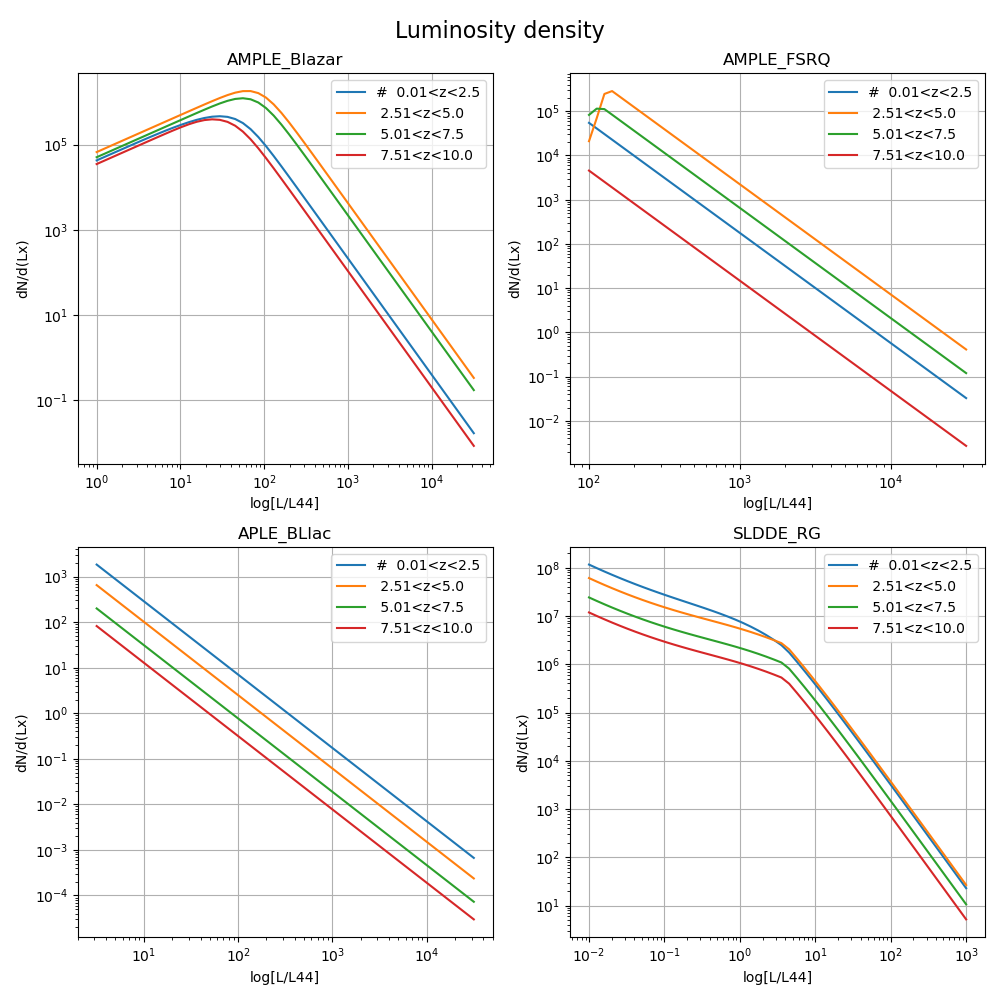
\includegraphics[width = \textwidth]{Luminosirt density.png}
    \caption{Luminosity density for the four different classes of AGNs. The different classes are defined in the title as well as the chosen LF model.}
    \label{fig:LD}
\end{figure}

In \ref{fig:LD} one can see the luminosity density for the four different classes of AGNs. The distribution are 
seperated into four bins of redshift ($0<z<2,2<z<4,4<z<6,6<z<8$). This is done to illuminate the evolution of the different classes at different 
epochs

For the blazar population in the top left of image \ref{fig:LD} one sees a clear break around $10^{46}$ erg/s. This break indicate that there is a distribution
around this value and that the most common blazar will be found around this energy level. The distribution also shows a clear evolution in time. wheras the earliest epoch
and the current epoch both have the fewest number of sources. This evoltion will become more clear in the next section.

For the FSRQs and for the BL Lacs one sees a different distribution. Where one sees more sources as we go to lower energies. The break luminosity for FSRQs 
is very close to the edge of the luminosity range and is almost nor visible. The Bl Lacs on the other hand do not have a break 
due to their representation as a simple power law.  

For the Radio galaxy population one sees a different distribution. Here the distribution has a break at $10^{45}$ erg/s and then continues to 
decrease but with a harder slope. To explain the hardening of the slope one might turn to classification issues with AGNs but it is not clear.


\subsubsection{Density distribution}

In addition to the luminosity distribution one can also calculate the number density of the different classes of AGNs. This is done by integrating the
differential luminosity function over all luminosities. This will illuminate the evolution of the different classes of AGNs in terms of redshift. The integral is given as

\begin{equation}
    \frac{dN}{dz} = \int_{L_{\text{min}}}^{L_{\text{max}}} \frac{\Psi(L, V(z))}{dL} \frac{dV(z)}{dz} dL
\end{equation}

Here again we seperate into luminosity bins in order to see the evolution seen in the previous chapter. This might seem redundent but
it gives one a stronger intution of the number of objects that are most common at which epoch, and their luminosity. 





\begin{figure}
    \centering
    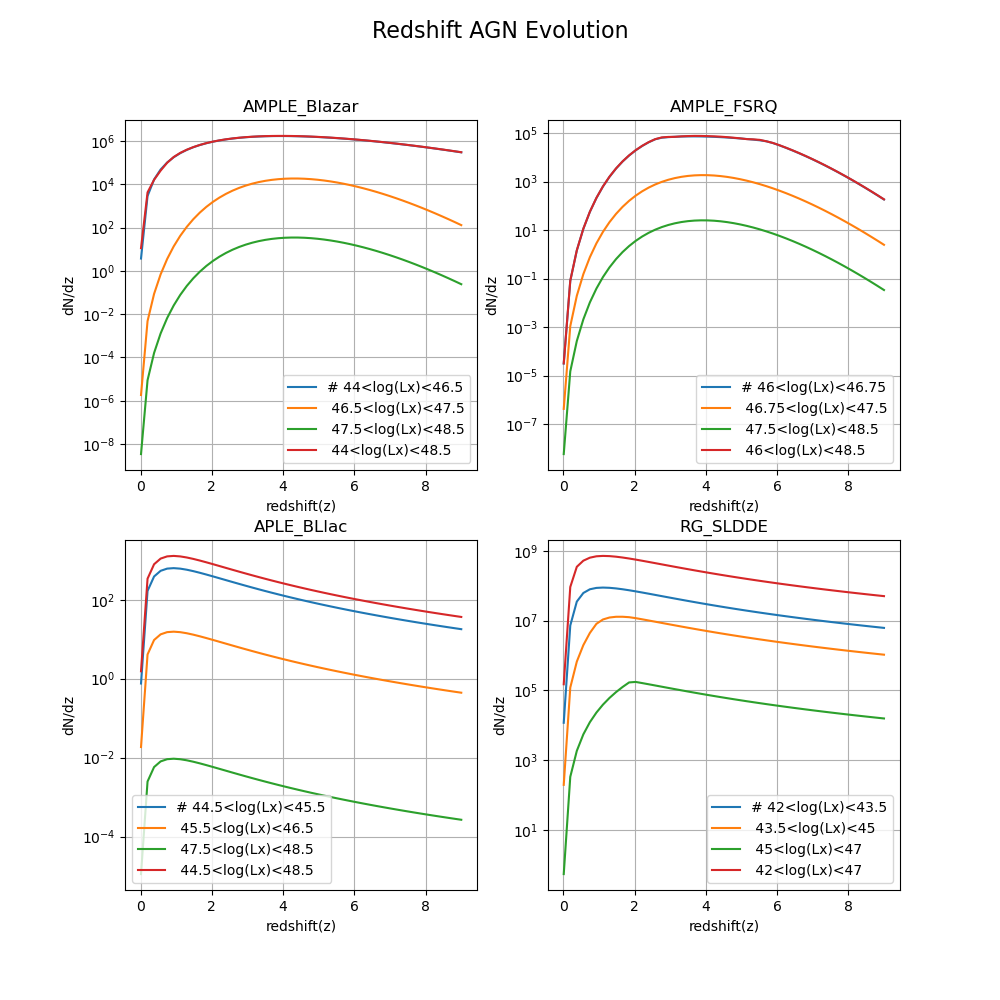
\includegraphics[width = \textwidth]{Redshift AGN Evolution.png}
    \caption{Number evolution in terms of redshift for the four different classes of AGNs. The different classes are defined in the title as well as the chosen LF model.}
    \label{fig:ND}
\end{figure}



In \ref{fig:ND} one sees the number evolution of the different classes of AGNs. The evolution is seperated into four bins of redshift ($0<z<2,2<z<4,4<z<6,6<z<8$).

For the blazar population in the top left of image \ref{fig:ND} one sees a clear trend with a top point around redshift $z=5$. 
This is then the epoch where most blazars are present, but it takes a quite uniform shape over all time.


For the FSRQs the evolution is quite linked to the blazard population. This is expected since FSRQs and BLlacs are thought to be 
sub groups of the bigger blazar group. The evolution also peaks around redshift $z=5$ but is less uniform over time. There is a bigger drop 
in numbers in the earlier and more recent epochs. 

For Bllacs the distribution is very different. Here the peak comes more aorund redhsift $z=2$ and then drops of quite rapidly for older epochs.
This evolution is very fascinating since it could contain information about the evolution of the universe and the creation of these 
objects. 

For the radio galaxies the trend is similar to the Bllacs. The peak of the time evolution is at more recent epoch ($z=1$) and the peak is 
luminosity dependent. The peak of the most luminous radio galaxies are at higher redshift than the less luminous ones.In addition from source .... one can find
the evolution comparable to the evolution of the star formation rate. This is interesting since it might indicate that the two are linked.


The representation of these objects can also be shown by their density distribution. By simply dividing the total number density by the comoving volume one can
find the density of these objects in the universe. By looking at figure \ref{fig:DD} one can see the density distribution and the effects this has on our interpretation of these objects.

The evolution is similar to that of the total number evolution, but one highlights the biggest difference between the groups. That one groups namely the Bllacs and the radio galaxies
are increasing in density when looking at lower redshifts and the other two groups are decreasing. This is a very interesting result since it might indicate that the two groups are 
a product of a different conditions in the universe, for example the totalt density of matter. 



\begin{figure}
    \centering
    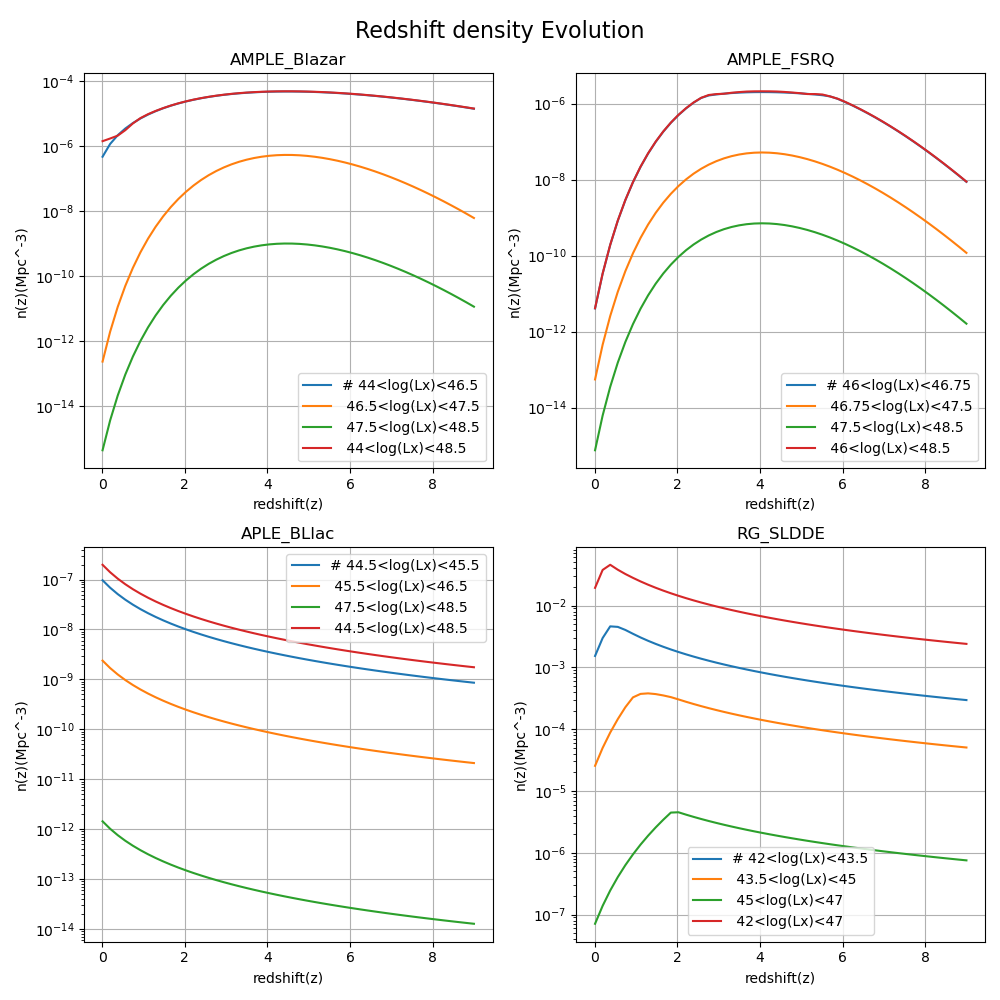
\includegraphics[width = \textwidth]{Redshift density Evolution.png}
    \caption{Density distribution for the four different classes of AGNs. The different classes are defined in the title as well as the chosen LF model.}
    \label{fig:DD}
\end{figure}



\subsubsection{Expected luminosity evolution}
Another point of interest is the exptect luminosity of an object at different redshift. This is important since it will directly relate to the 
power output of the different epochs and from this one can calcualte an expected emmisitivty of the different classes of AGNs. 
The expected luminosity of each group can be calcualted with the following formula. 

\begin{equation}
    \langle L \rangle = \frac{\int_{L_{\text{min}}}^{L_{\text{max}}} L \frac{\Psi(L, V(z))}{dL} \frac{dV(z)}{dz} dL}{\int_{L_{\text{min}}}^{L_{\text{max}}} \frac{\Psi(L, V(z))}{dL} \frac{dV(z)}{dz} dL}
\end{equation}

The different luminosity ranges are the same as before and are given in table \ref{tab:lum_range}. The results are shown in figure \ref{fig:EL}.

\begin{figure}
    \centering
    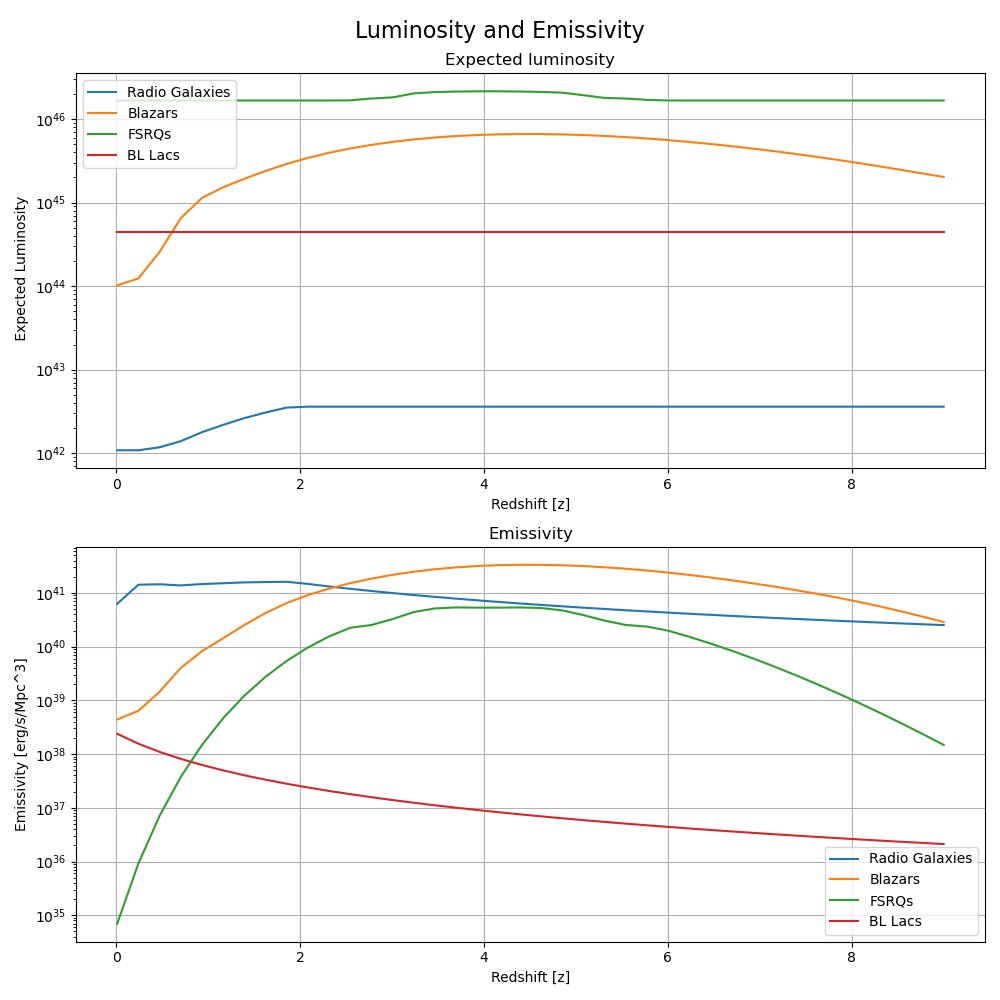
\includegraphics[width = \textwidth]{Luminosity and Emissivity.png}
    \caption{Expected luminosity and emmisivity for the four different classes of AGNs. The different classes are defined in the title as well as the chosen LF model.}
    \label{fig:EL}
\end{figure}

The expected luminosity shown at the top is a great reminder of the different classes. Here one sees that FSRQs are inndeed the most luminous part of a blazar AGN and 
that they represent some of the most luminous objects in the universe. The trend for FSRQs is also very flat with a small bump at the middle epochs. 

The Bllacs on the other hand are not as luminous as the FSRQs but are still very luminous. 
The trend for the Bllacs is a very flat evolution indicating that the produced Bllacs although fewer at earlier epochs are still 
of similar magnitudes.

The group with the biggest varaibility in expected Luminosity is the blazars. Here one sees a curve over the epochs with a peak around redshift $z=5$. 
This indicates that the produced blazars in newer epochs are less luminous on averge. A similar results obtained from the luminsoity distribution in figure \ref{fig:LD}.
The evolution of the expected luminosity might be indicative of a badly defiend gorup of objects since one usually distinctions objects based on their luminosity.

The radio galaxies are the least luminous of the four groups and have a very flat evolution. This is expected since the radio galaxies are not as luminous as the blazars.

The emmisivity shown at the bottom in figure \ref{fig:EL} shows a more intersting evolution. The figure shows the output of energy per unit volume per unit time. In other words 
how much energy these objects are producing and by extension which objects would be relevant at different epochs due to their dominance over the others.
The most interesting point is around redhsift $z=2$ where the emmisivity of the radio galaxies overtake the dominant blazars. This change would in theory make
a big splash in the observables here on earth should these objects be the origin of the UHECRs and neutrinos. 



\section{UHECRS emmisivity}
With the calculated emmisivity for the different groups there is now possibility to look very briefly into the possibility of AGNs being the origin of UHECRs. The 
reasoning is quite crude but in order for the AGNs to be the origin of UHECRs they must be able to produce the necessary energy. 

According to .... the energy density of UHECRs is given as $3*10^{44}\frac{erg}{Mpc^3yr}$ ....

In order to estimate the sources of these UHECRs and based on the limit of how close an UHECR could be produced to earth one can calculate the emmisivity needed to produce these UHECRs.
By estimating the emmisivity produced from our sources at a very low redshift (i.e $z=0.01$) one can then calculate emmisitivty of our sources and compared to the required emmisivity.



\subsection{Galaxy evoltuion}
\subsection{AGN evolution}
\subsubsection{Luminosity distribution}
\subsubsection{Density distribution}


\end{document}
